% Transformer 4 windings orig
% Author: Reto Christen
\documentclass[border = 200pt]{standalone}
\usepackage[landscape]{geometry}
\usepackage{tikz}
\usepackage{color}
\usetikzlibrary{circuits.ee.IEC, arrows}

%%%%%%%% Schaltzeichen AC source%%%%%%%%%%%%%
\tikzset{circuit declare symbol = AC source}
\tikzset{AC source IEC graphic/.style={
    circuit symbol lines,
    circuit symbol size=width 2 height 2,
    shape=generic circle IEC,
    /pgf/generic circle IEC/before background={
    \pgfpathmoveto{\pgfpoint{-0.8pt}{0pt}}
    \pgfpathsine{\pgfpoint{0.4pt}{0.4pt}}
    \pgfpathcosine{\pgfpoint{0.4pt}{-0.4pt}}
    \pgfpathsine{\pgfpoint{0.4pt}{-0.4pt}}
    \pgfpathcosine{\pgfpoint{0.4pt}{0.4pt}}
    \pgfusepath{stroke}
    },
    transform shape, draw
  }
}
\tikzset{circuit ee IEC/.append style=
  {set AC source graphic = AC source IEC graphic}
}
%%%%%%%%%%%%%%%%%%%%%%%%%%%%%%%%%%%%%%%%%%%%%%%

%%%%%%%%%%% Spannungspfeile %%%%%%%%%%%%%%
\tikzset{
  Pfeil/.style={thick,shorten >=#1,shorten <=#1,->,>=latex}, % für Peile
  UPfeil/.style={blue,Pfeil=#1,font={\sffamily\itshape}},% für Spannungspfeile
  IPfeil/.style={red,Pfeil=#1,font={\ttfamily\itshape}} % für Strompfeile
}
%%%%%%%%%%%%%%%%%%%%%%%%%%%%%%%%%%%%%%%%%

\definecolor{green}{rgb}{0, 1, 0}
\definecolor{qdance}{rgb}{1,0.5,0.15}

\begin{document}
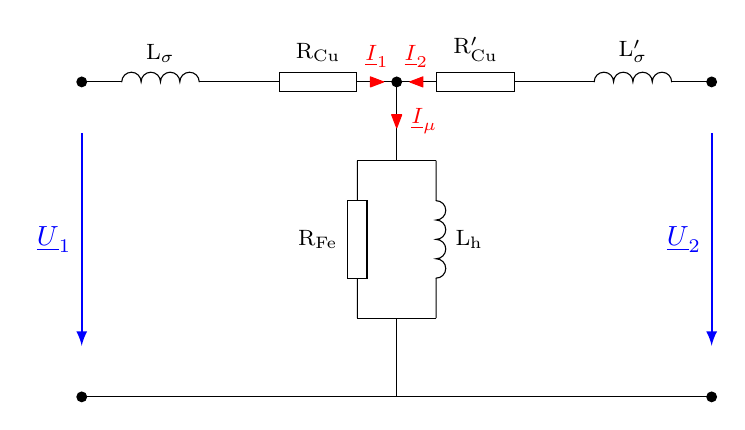
\begin{tikzpicture}[circuit ee IEC, font=\sffamily\footnotesize]
 
 
% % main resistor and inductor
\node[contact] at (0,0) {};
\draw (0,0) to [inductor={info={$\mathrm{L_\sigma}$}}] (2,0);
\draw (2,0) to [resistor={info={$\mathrm{R_{Cu}}$}}] (4,0);
\node [contact] at (4,0) {};
\draw (4,0) to [resistor={info={$\mathrm{R'_{Cu}}$}}] (6,0);
\draw (6,0) to [inductor={info={$\mathrm{L'_\sigma}$}}] (8,0);
\node [contact] at (8,0) {};

\draw (3.5,-3) to [resistor={info={$\mathrm{R_{Fe}}$}}] (3.5,-1);
\draw (4.5,-1) to [inductor={info={$\mathrm{L_h}$}}] (4.5,-3);
\draw[] (4,0) -- (4,-1){};
\draw[] (3.5,-1) -- (4.5, -1){};
\draw[] (4,-3) -- (4,-4){};
\draw[] (3.5,-3) -- (4.5, -3){};

\node [contact] at (0,-4) {};
\node [contact] at (8,-4) {};
\draw[] (0,-4) -- (8,-4) {};

% Pfeile
\draw[UPfeil=-1em](0,-1) -- node [xshift=-1em]{$\underline{U}_1$}(0,-3);
\draw[UPfeil=-1em](8,-1) -- node [xshift=-1em]{$\underline{U}_2$}(8,-3);

\node[current direction={red, info={[red]\texttt{\itshape{$\underline{I}_1$}}}}] at (3.75,0) {};
\node[current direction'={red, info'={[red]\texttt{\itshape{$\underline{I}_2$}}}}] at (4.25,0) {};
\node[current direction={red, info={[red]\texttt{\itshape{$\underline{I}_\mu$}}}}, rotate=270] at (4,-0.5) {};


\end{tikzpicture}
\end{document}
